\section{Introduction}
Attitude estimation is the process of estimating the orientation of an aerospace vehicle with respect to an intertial frame of reference.

Usually, in air navigation, attitude is determined with 3 angles:
\begin{itemize}
\item \textbf{Yaw}: angle respect to true north. Heading.
\item \textbf{Pitch}: angle of the nose respect to the horizon. Angle of attack.
\item \textbf{Roll}: angle of the wings respect to the horizon. Bank.
\end{itemize}
\begin{figure}[h]
\centering
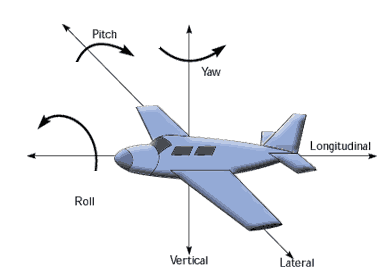
\includegraphics[width=0.6\textwidth]{figures/attitude.png}
\caption{Attitude angle axis on airplane}
\label{fig:attitude}
\end{figure}

To perform attitude estimation some sensors are needed. The most commonly used in inertial navigation systems (INS) are:
\begin{itemize}
\item Accelerometer: gives direction of gravity.
\item Gyroscope: gives rate of turn.
\item Magnetometer: gives direction of magnetic north.
\end{itemize}

The goal of this project is to assemble a HW device capable of measure sensor data that later, applying an Extended Kalman Filter, is capable of estimating the attitude of the setup.